\documentclass{standalone}
\usepackage{preset}
\begin{document}
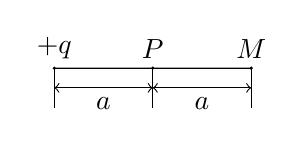
\begin{tikzpicture}[x=25mm,y=25mm]
	\draw[fill=black](0,0)circle(.005)node[above]{$+q$}--(.5,0)circle(.005)node[above]{$P$}--(1,0)circle(.005)node[above]{$M$};
	\foreach \x in{0,.5,1}{
		\draw(\x,0)--++(0,-.2);
	}
	\draw[<->](0,-.1)--node[below]{$a$}+(.5,0);
	\draw[<->](.5,-.1)--node[below]{$a$}+(.5,0);
\end{tikzpicture}
\end{document}
